\documentclass[10pt]{article}
\usepackage{parskip}
\usepackage[utf8]{inputenc}
\usepackage[left=2.00cm, right=2.00cm, top=2.00cm, bottom=2.00cm]{geometry}
\usepackage[spanish]{babel}
\usepackage{graphicx,subfig}
\usepackage{fancyhdr}
\graphicspath{{Imagenes/}}
\usepackage{enumerate} 
\usepackage{multicol}
\begin{document}


\pagestyle{fancy}
\cfoot{}


%Cabeceras
\rhead{Conocimiento y manejo del Osciloscopio}
\lhead{}

%Portada
\begin{titlepage}
	\newgeometry{
		left=25mm,
		right=25mm,
		top=5mm,
		bottom=30mm,
		headheight = 0 mm
	}

	\begin{figure}[t]
		\subfloat{
\includegraphics[width=0.15\textwidth]{Logo_IPN}}
		\hspace{0.7\textwidth}
		\subfloat{
\includegraphics[width=0.22\textwidth]{LogoEsime}}
	\end{figure}

	\centering
	{\bfseries\Huge Instituto Politécnico Nacional. \par}
	\vspace{1cm}
	{\scshape\Large Ingeniería en Comunicaciones y Electrónica. \par}
	\vspace{0.3cm}
	{\scshape\Large Laboratorio de Electricidad y Magnetismo.  \par}
	\vspace{1cm}
	{\scshape\Huge LAS ONDAS \par}
	\vspace{1cm}
	{\itshape\Large Conocimiento y manejo del Osciloscopio. \par}
	{\Large 2CM13\par}
	\vfill
	{\Large Autores: \par}
	{\Large Daniela Elizabeth Pérez Vargas. \par}
	{\Large Jesús Martinez Amac. \par}
	{\Large José Emilio Hernández Huerta. \par}
	{\Large Nataly Bejarano Garduño..\par}
	{\Large Uriel Grimaldi Díaz.  \par}
	\vfill
	{\Large Mayo 2023. \par}

\end{titlepage}

\tableofcontents
\newpage




\section{Resumen.}
Por medio de instrumentos especializados se observo el comportamiento de multiples funciones de onda por medio de un osciloscopio el cual muestra en pantalla de una forma grafica al igual que se aprendera a utilizar un generador de funciones de onda para mostrarlas en la pantalla del osciloscopio.

\begin{multicols}{2}
\section{Objetivo.}
El alumno identificara las perillas y botones requeridos para un empleo básico del osciloscopio, calibrara el osciloscopio en frecuencia y voltaje, efectuara la medicion de tensiones directas y alternas y por ultimo realizara la medicion de la frecuencia y periodo de una señal.

\section{Introducción.}
Las funciones de ondas nos ayudan a comprender de mejor forma los comportamientos de algunos sistemas un ejemplo de esto seria en la reparacion de un celular al poder medir el consumo de energia con respecto al tiempo nos proporciona informarcion util como; porque no llega a prender, componentes dañados, corto circuitos, ect. También es de gran ayuda para poder estudiar de mejor forma el campo de la electricidad. Por eso es importante que el estudiante aprenda a manejar de forma correcta un osciloscopio.


\section{Marco teórico.}
El Generador de señales: Un Generador de Señales es un instrumento de laboratorio que permite crear electrónicamente diferentes tipos de señales a diferentes frecuencias y diferentes amplitudes. \\
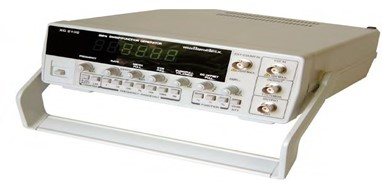
\includegraphics[width=0.1\textwidth]{Imagenes/Marco Teorico/Imagen1}\\
Señal Sinusoidal\\
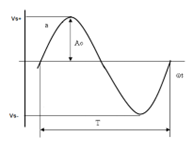
\includegraphics[width=0.1\textwidth]{Imagenes/Marco Teorico/Imagen2}\\
Señal Triangular\\
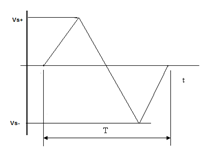
\includegraphics[width=0.1\textwidth]{Imagenes/Marco Teorico/Imagen3}\\
Señal Cuadrada\\
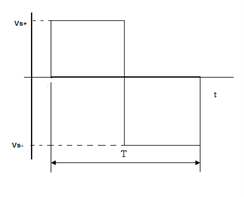
\includegraphics[width=0.1\textwidth]{Imagenes/Marco Teorico/Imagen4}\\
En donde:
T = Periodo de la señal. 
Vs+ = Voltaje positivo Máximo
Vs- = Voltaje negativo Máximo
A0 = Amplitud de la señal.
Es importante recordar que la frecuencia de la señal (en Hz) está dada por:
F= 1/T
Y que el Voltaje Pico a Pico o Vpp está dado por:
$ Vpp= (Vs+)  (Vs-) $
Los generadores de señales tienen un rango de frecuencia y amplitudes de funcionamiento y permiten entre otras funciones, calibración de equipos, pruebas a sistemas de audio, pruebas a servo motores.
El Osciloscopio es un aparato de medición que es capaz de mostrar señales eléctricas variantes en el tiempo. Además de la observación de estas señales con el osciloscopio es posible realizar análisis de frecuencia de la señal, determinar transitorios o cambios dinámicos en una señal.
Un osciloscopio esta constituido básicamente en los siguientes subsistemas.
1.- Tubo de rayos catódicos (CRT)
2.- Amplificadores verticales y horizontales
3.- Circuito Base de tiempo
4.-Fuentes de potencia
El osciloscopio es un equipo que sirve para visualizar formas de onda de TENSIÓN de un circuito. Las formas de onda las representan en dos ejes: el eje de abscisas representa tiempo y el eje de ordenadas representa tensión.\\

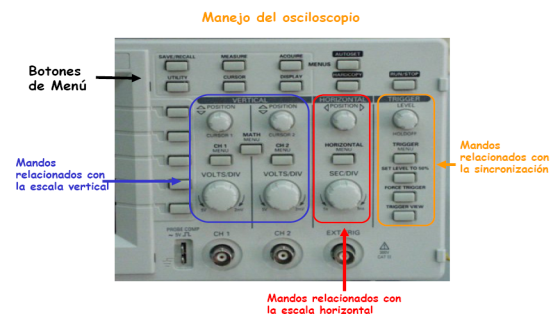
\includegraphics[width=0.1\textwidth]{Imagenes/Marco Teorico/Imagen5 pero usa el tuyo .png}\\
Las escalas de ambos ejes son modificables por el usuario. La pantalla está dividida en cuadrículas y lo que el usuario elige es el valor de cada una de esas cuadrículas.
Ejemplo de la pantalla del osciloscopio:\\

\includegraphics[width=0.1\textwidth]{Imagenes/Marco Teorico/Imagen6}\\
Cada línea horizontal representa un voltaje que puede ser variado con las perillas del osciloscopio ( Volts / Division)
Cada línea Horizontal representa una escala de tiempo que puede ser variada con la perilla del osciloscopio ( Time/ Division)




\section{Descripción de materiales.}
\subsection{Osciloscopio}

Un osciloscopio es un instrumento de medición, el cual representa una gráfica de amplitud en el eje vertical y tiempo en el eje horizontal.

\begin{center}
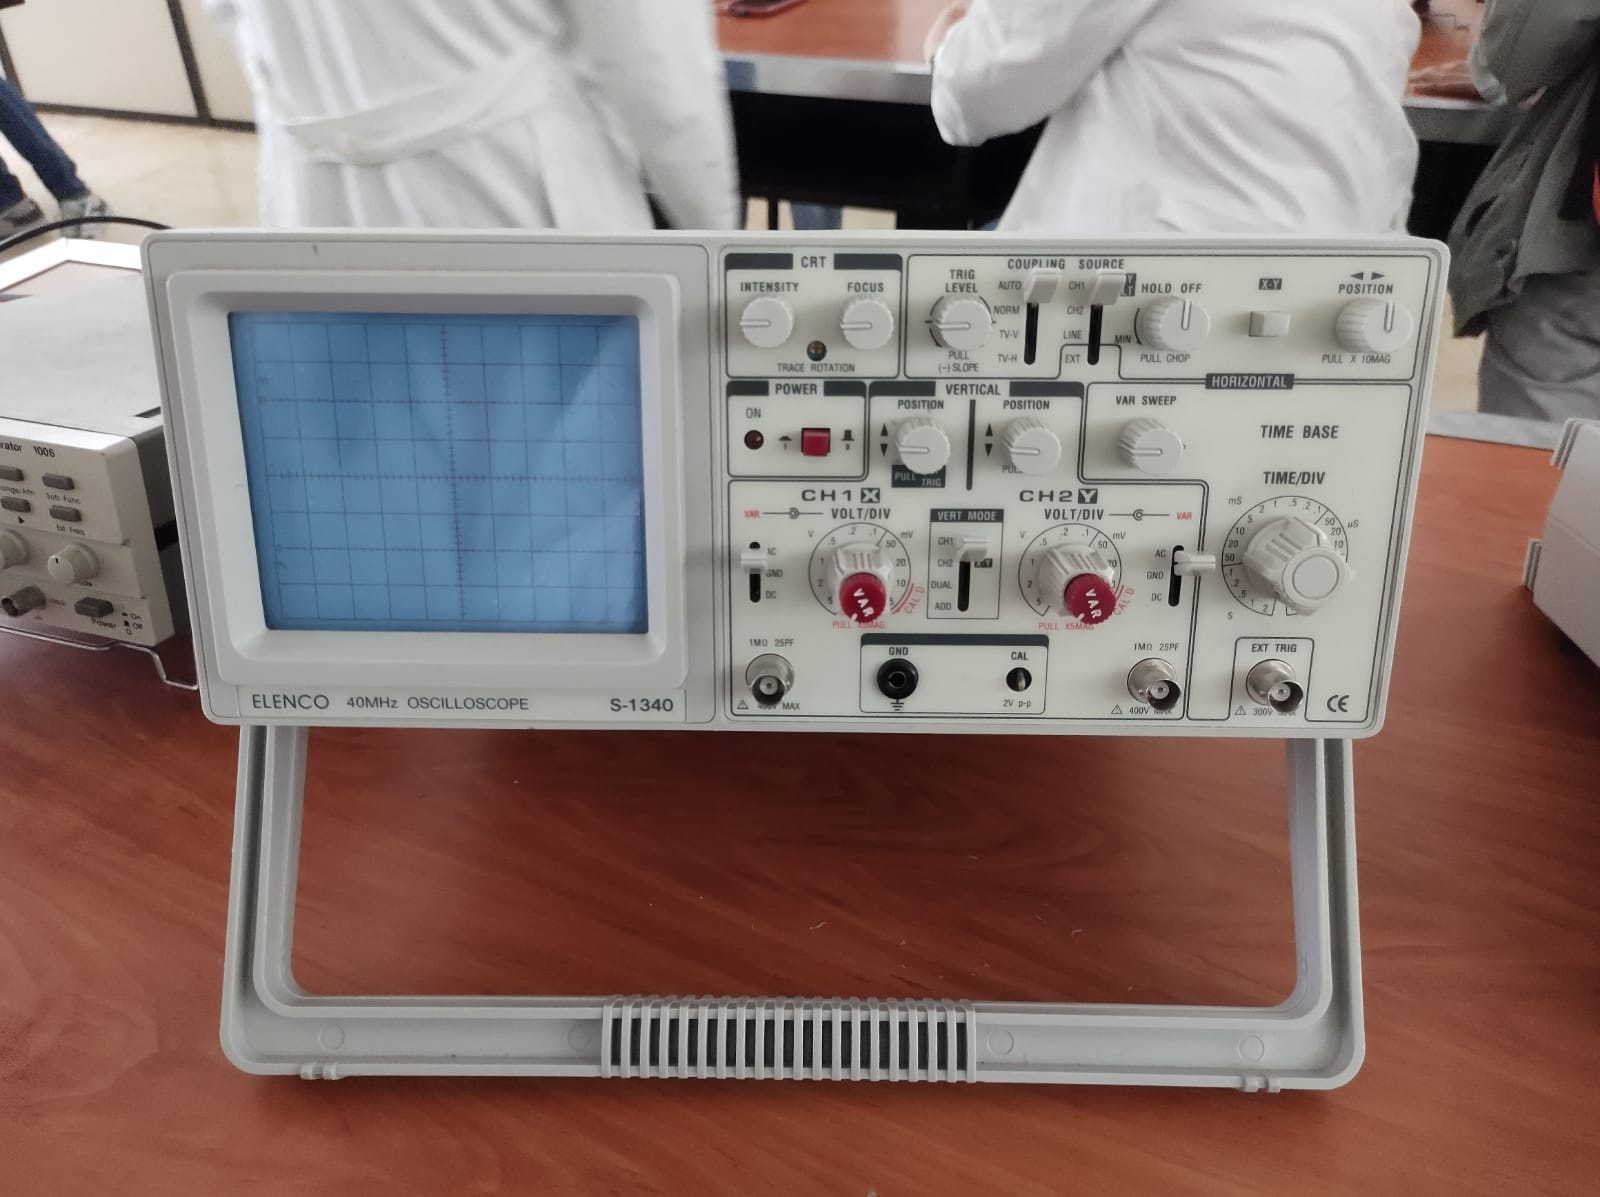
\includegraphics[scale=0.1]{Imagenes/osciloscopio.png}\\
Reconocimiento del Osciloscopio.
\begin{enumerate}
\item La marca del Osciloscopio es Elenco.
\item Cuenta con 3 canales el equipo.
\item Cuenta con 10 posiciones en la perilla VOLTS/DIV.
\item Los rangos con los que cuenta en la perilla VOLTS/DIV en V son: 5,2,1,.5,.2,.1, y en mv son: 50,20,0,5.
\item Cuenta con 23 posiciones la perilla TIME/DIV.
\item Los rangos con los que cuenta en la perilla TIME/DIV S son: 2,1,.5,.2,.1, en ms son: 50,20,10,5,2,1,.5,.2,.1, y en ns son: 50,20,10,5,2,1,.5,.2,.1.
\end{enumerate}
\end{center}

\subsection{Generador de funciones.}

\begin{center}
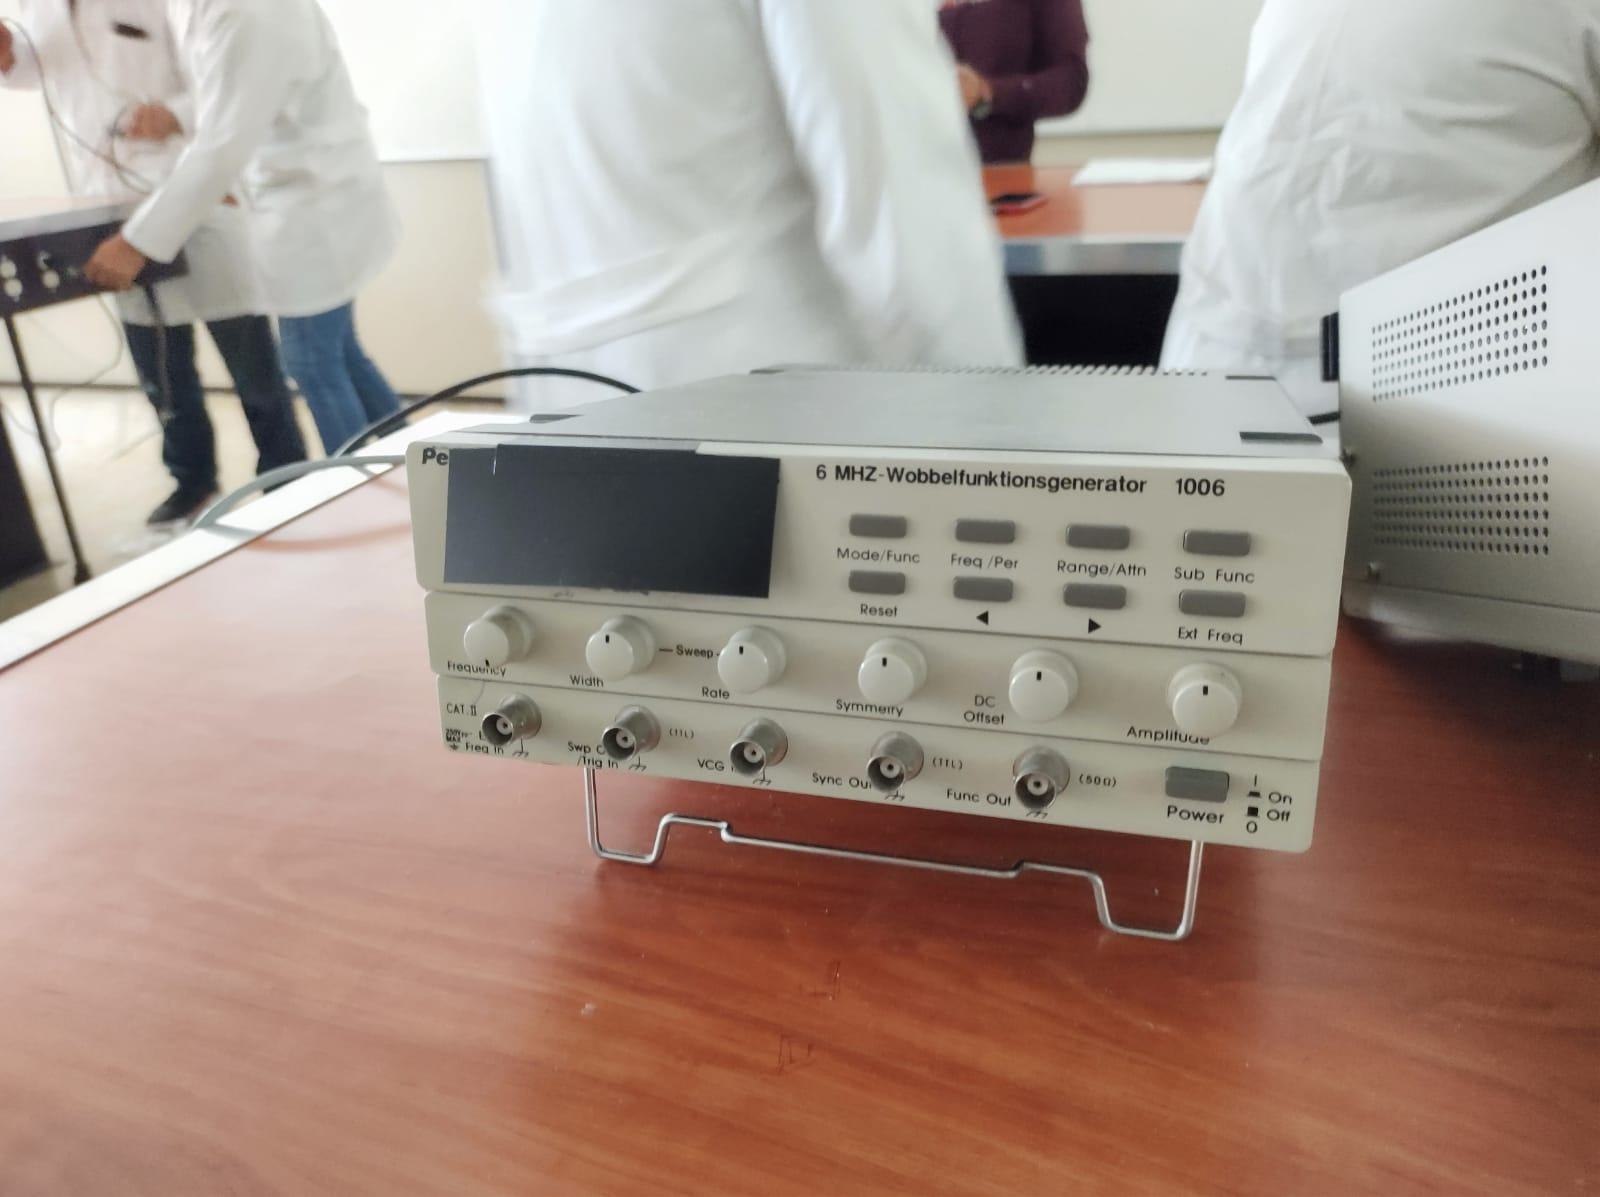
\includegraphics[scale=0.1]{Imagenes/generador.png}\\
Reconocimiento del Generador de funciones
\begin{enumerate}
\item Cuenta con 5 canales los cuales se llaman:Freq In, Trig In, VCG In, Sync Out y Func Out.
\item El canal 5 llamado func Out es el canal de salida.
\item Genera patrones de señales periódicas o no periódicas tanto analógicas como digitales.
\end{enumerate}
\end{center}

\subsection{Cable BNC - Caimán.}

\begin{center}
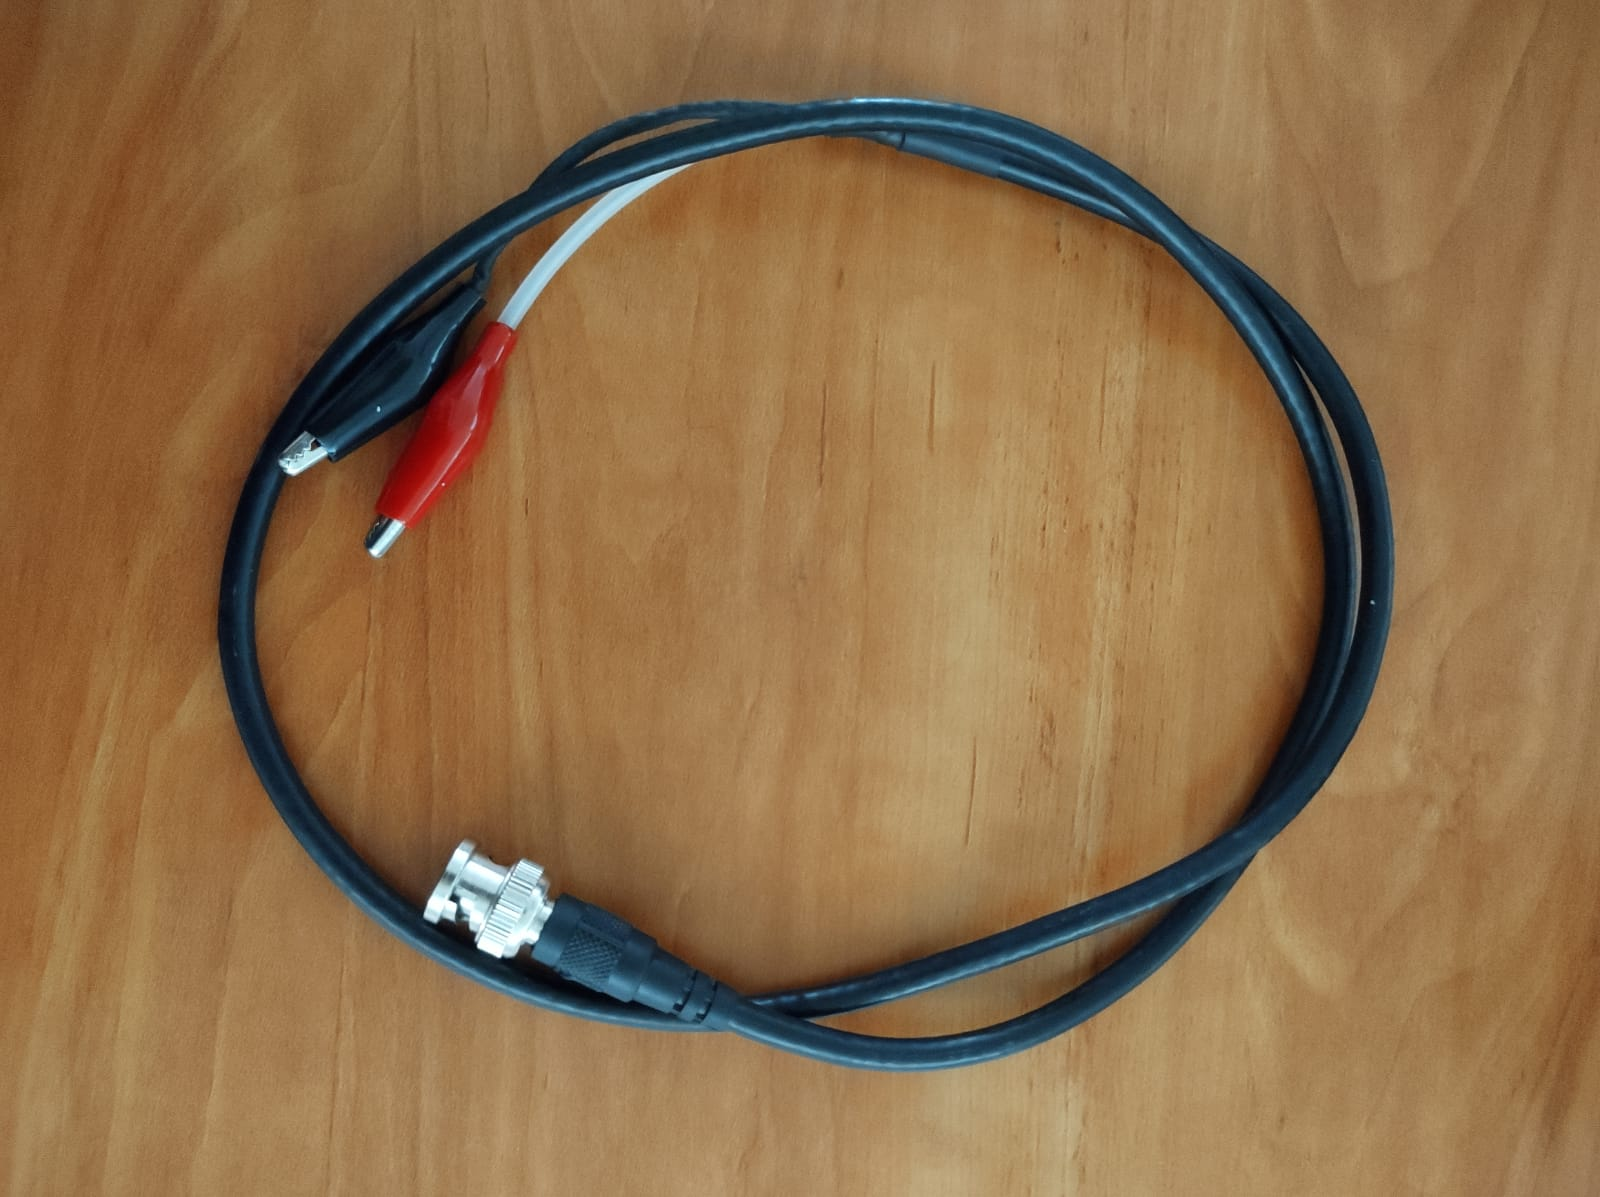
\includegraphics[scale=0.1]{Imagenes/caimanes.png}\\
Reconocimiento del cable BNC - Caimán.
\begin{enumerate}
\item Cuenta con dos caimanes.
\item El caiman de color rojo es positivo.
\item El caiman de color negro es negativo.
\item Cuenta con un cable BNC, en el cual se conecta con los canales CH1 ó CH2 del Osciloscopio.
\end{enumerate}
\end{center}

\subsection{Punta de prueba.}

\begin{center}
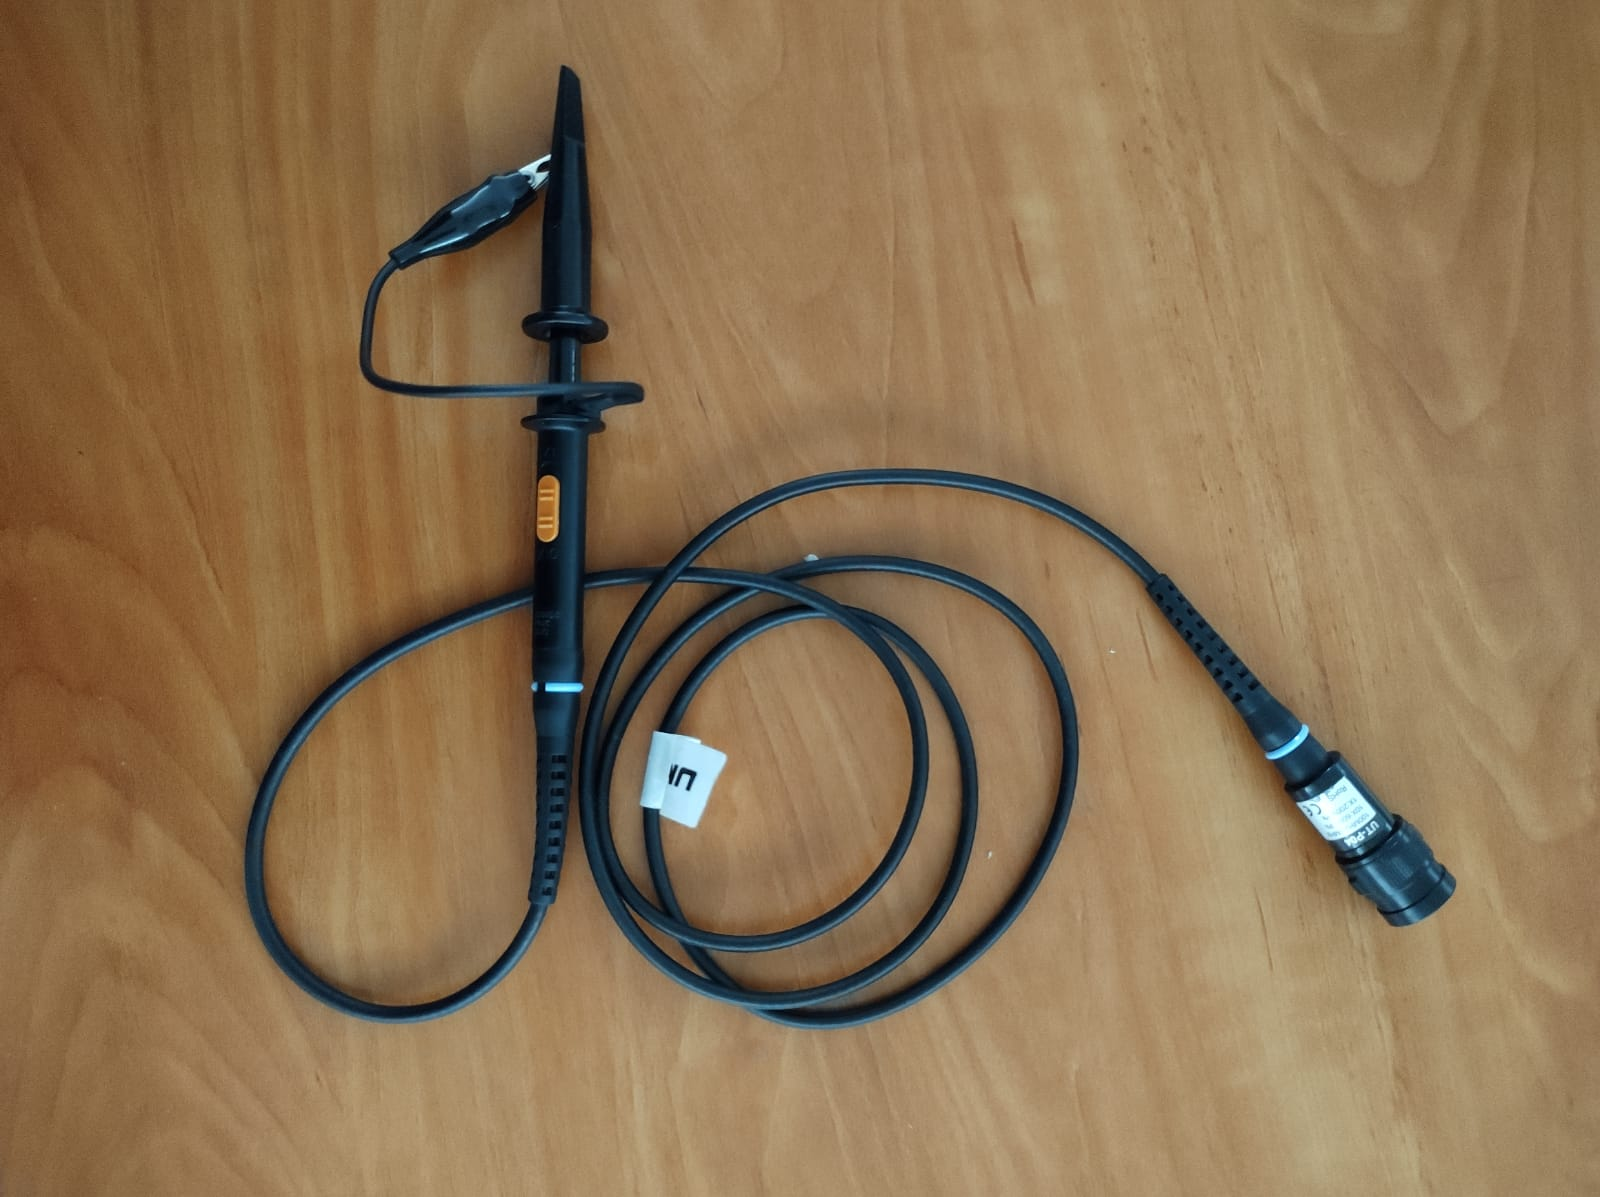
\includegraphics[scale=0.1]{Imagenes/prueba.png}\\
Reconocimiento de punta de prueba.
\begin{enumerate}
\item Cuenta con un cable BNC en el cual se conecta em los canales CH1 ó CN2 del Osciloscopio.
\item Cuenta con un gancho cubierto con una goma el cual le  da señal al Osciloscipo, y ese gancho hace la funcion del caiman color rojo ya que ambos son positivos.
\item Cuenta con un caiman de color negro el cual es negativo.
\end{enumerate}
\end{center}

\subsection{Bateria.}

\begin{center}
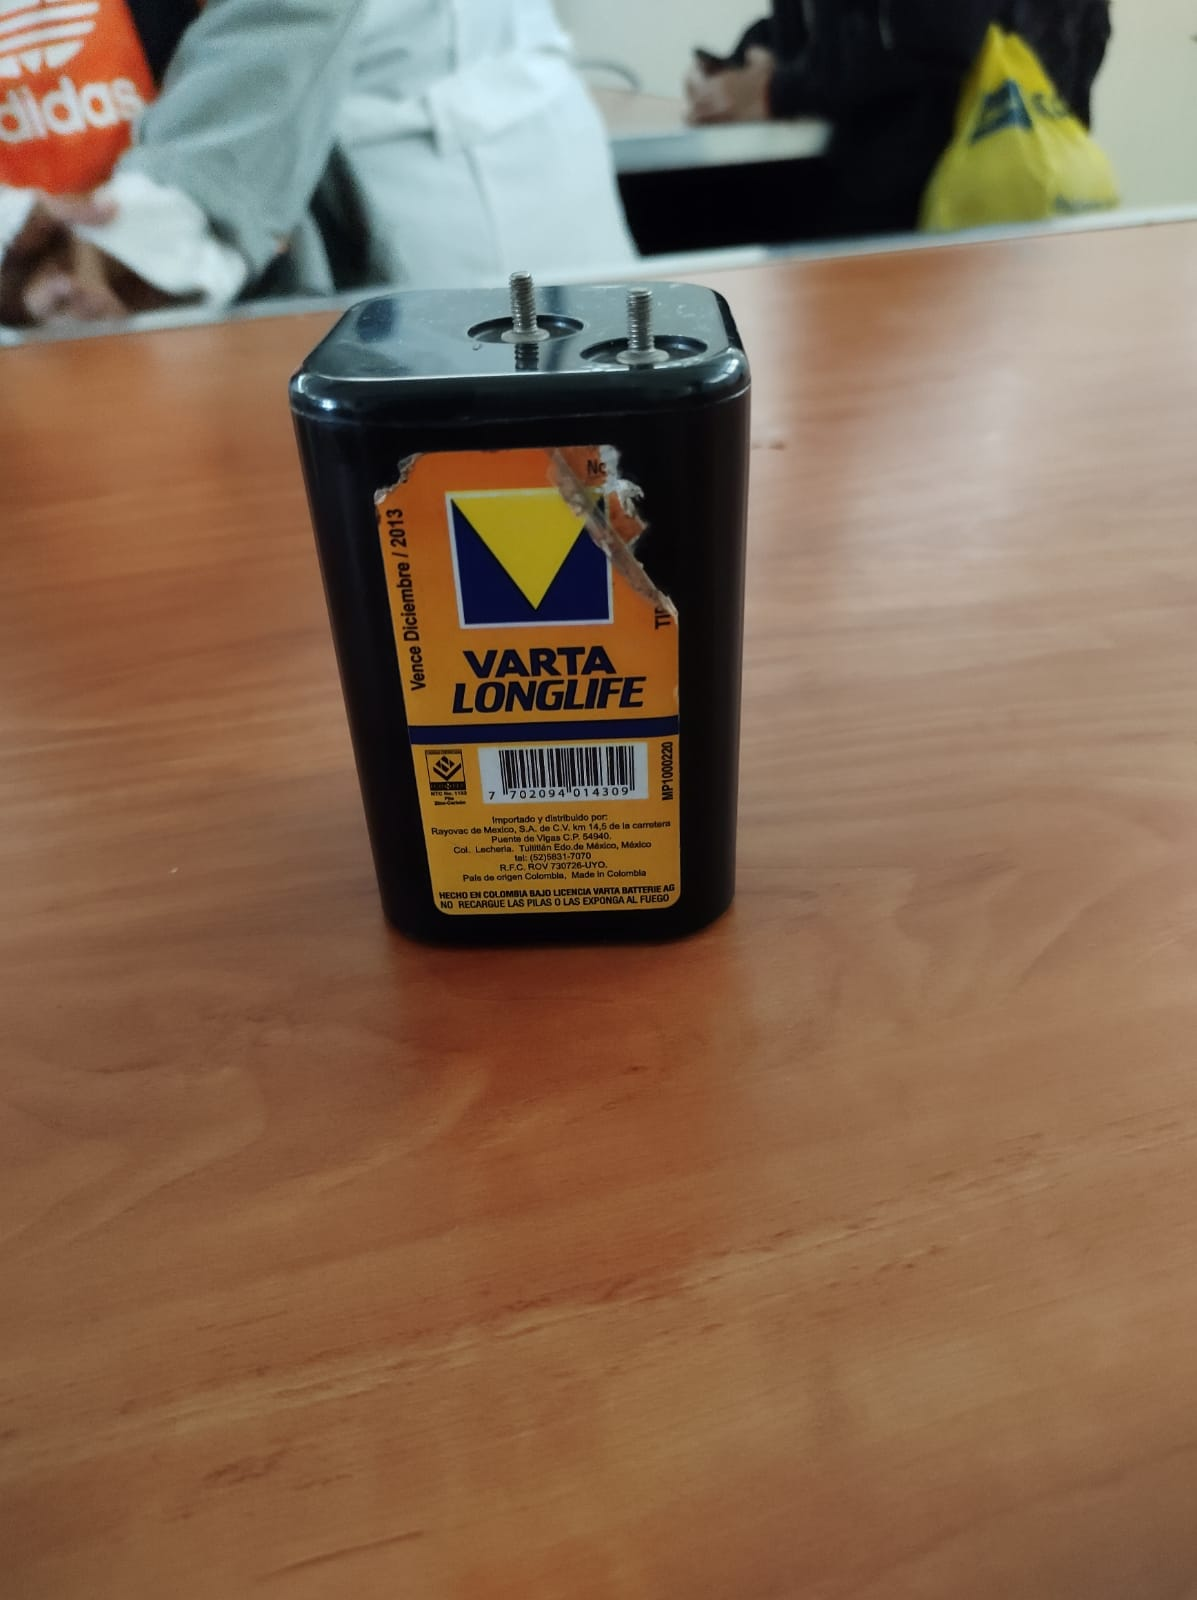
\includegraphics[scale=0.1]{Imagenes/bateria.png}\\
Reconocimiento de la Bateria.
\begin{enumerate}
\item La marca de la bateria es VARTA LONGLIFE.
\item La bateria es de 9V.
\item Cuenta con un catodo positivo.
\item Cuenta con anodo negativo.
\end{enumerate}
\end{center}
 

\section{Desarrollo experimental.}
Primero calibramos el osciloscopio conectando la punta de prueba en el espacio indicado para su calibracion despues giramos las perillas para que todo este en su correcta posicion, despues prendimos el generador de funciones y empezamos a darle diferentes amplitudes y frecuencias, para despues conectar una bateria de 3 Volts la cual arrojaba una grafica lineal.
\section{Análisis y resultados.}
Las funciones de onda creadas por el generador pueden ser escaladas tando de la fuente como del osciloscopio dando un mayor rango de presicion y control en las mediciones, tambien otro punto importante a destacar es que la bateria muestra una linea recta la cual a partir del punto de origen marca 3 linear hacia arriba es porque esta bateria es de 3 volts y al ser una medicion la cual cambiara con el tiempo pero mucho despues lo vemos como una constante.

\section{Conclusiones.}
\subsection{José Emilio Hernández Huerta}
Podemos apreciar como desde el movimiento de un punto individual podemos crear una serie de lineas las cuales se me hacen muy increíbles, desde pulsos, funciones triangulares, senoidales e incluso los figuras que se pueden crear superponiendo las ondas de 2 generadores a un mismo osciloscopio. El osciloscopio nos brinda la capacidad de observar y medir diferentes parámetros de una señal, como amplitud, frecuencia, forma de onda, tiempo de subida, entre otros. Su pantalla nos muestra gráficamente la representación temporal de la señal, lo que facilita la identificación de irregularidades, distorsiones o problemas de funcionamiento.

Además de su utilidad en el análisis de señales, el osciloscopio también nos permite realizar mediciones precisas y comparativas entre diferentes señales, lo que resulta esencial en la depuración y verificación de circuitos electrónicos. Nos proporciona una visión detallada de cómo se comporta una señal en el tiempo y nos ayuda a comprender mejor su naturaleza y características.

\subsection{Jesus Martinez Amac}
Aprendí que hay Osciloscopios analógicos ó digitales, en ambos tienen sus ventajas o sus inconvenientes y es un instrumento que traza graficas en el plano de la X y la Y, y da una señal con respecto al otro o bien con respecto al tiempo, también aprendí que en el eje de la Y (Vertical) es la que recibe la señal procedente que procede de la tensión que está siendo examinada obteniéndose de un punto luminoso en el sentido vertical, y la señal en el eje de la X (Horizontal) procede del generador de una rampa lineal de voltaje,tambien aprendí que el instrumento es de empleo delicado, así que se debe de manejar de buena manera el manejo de los controles así para no dañar el instrumento.
Cómo mi conclusión , se que el Osciloscopio nos ayuda  para dar a  conocer la amplitud de un voltaje y su frecuencia, también sirve para captar y diferenciar las distintas corrientes alternas y a la principal, además, permite identificar fallos presentes en una señal.
\subsection{Nataly Garduño Bejarano}
Un osciloscopio es un instrumento de medición para la electrónica. Representa una gráfica de amplitud en el eje vertical y tiempo en el eje horizontal. Es muy usado por ingenieros en el campo de la electrónica. Frecuentemente se complementa con un multímetro, una fuente de alimentacón y un generador de funciones o arbitrario.
El osciloscopio presenta los valores de las señales eléctricas en forma de coordenadas en una pantalla, en la que normalmente el eje X (horizontal) representa tiempos y el eje Y (vertical) representa tensiones. La imagen así obtenida se denomina oscilograma. En osciloscopios análogos o de fosforo digital se suele incluir otra entrada o control, llamado "eje Z" que controla la luminosidad del haz, permitiendo resaltar o apagar algunos segmentos de la traza dependiendo de su frecuencia de repetición o velocidad de transicion en tiempo.
El osciloscopio digital la señal es previamente digitalizada por un conversor analógico digital. Al depender la fiabilidad de la visualización de la calidad de este componente, esta debe ser cuidada al máximo.
Las características y procedimientos señalados para los osciloscopios analógicos son aplicables a los digitales. Sin embargo, en estos se tienen posibilidades adicionales, tales como el disparo anticipado (pre-triggering) para la visualización de eventos de corta duración, o la memorización del oscilograma transfiriendo los datos a un PC. Esto permite comparar medidas realizadas en el mismo punto de un circuito o elemento. Existen asimismo equipos que combinan etapas analógicas y digitales.

\subsection{Perez Vargas Daniela Elizabeth}
Una conclusión sobre los osciloscopios es que son herramientas esenciales para medir y analizar señales eléctricas en diversas aplicaciones como ingeniería, electrónica y física. Permiten al usuario visualizar formas de onda de señal, medir voltajes y corrientes y observar el comportamiento de los circuitos a lo largo del tiempo. Esta información es crucial para diagnosticar problemas y verificar el rendimiento de los sistemas electrónicos. Además, el uso generalizado de osciloscopios digitales los ha hecho más accesibles, lo que permite que una gama más amplia de personas experimente con la electrónica y adquiera experiencia de primera mano en el análisis de señales. En general, no se puede subestimar la importancia de los osciloscopios, y siguen siendo una herramienta crítica para cualquier persona que trabaje con señales electrónicas.

\end{multicols}
\newpage
\clearpage
\begin{thebibliography}{0}
	\bibitem{}[Cabrera, J. L. (2006). Redes Locales. México: Alfa Omega.]
	\bibitem{}[ Felipe, R. J. (2011). Telecomunicaciones : historia y conceptos básicos . México: El colegio Nacional.]
		\bibitem{}[Manuel, H. M. (2004). Manual de telecomunicaciones. México: Alfaomega.]
		\bibitem{}[Stallings, W. (2004). Comunicaciones y redes de computadoras. Marid España: Pearson Prentice Hall.]
		\bibitem{}[Tanenbaum, A. (2011). Redes de Computadoras. Pearson.]
	
\end{thebibliography}

\end{document}

